\scanpage{8}
\figure{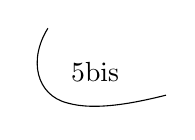
\begin{tikzpicture}[x=1cm,y=1cm]
\node at (.7,.45) {\mspage{5bis}};
\draw (.1,1.0) .. controls (-.15,.6) and (-.05,.15) .. (.35,.05) .. controls (.7,-.05) and (1.2,.05) .. (1.6,.15);
\end{tikzpicture}}
5. On peut aussi donner une condition d'\uline{existence} des $\pi_i$, liée aux conditions $(4.4)$. Pour ceci, on suppose que $\mathcal E$ est contenu dans un \unsure{sur-anneau|sous-anneau} gradué $\mathcal F$ [p.ex. \inserted{l'anneau} des endom. d'un $M^*$ comme dans 1.] pour lequel les $\pi_i$ satisfont $(1.1.)$ et les relations \unsure{correspondantes|correspondant} à $(1.3)$ (avec $\mathcal E$ remplacé par $\mathcal F$) sont satisfaites; \inserted{(et $(3.0)$: $\pi_i=0$ si $i\notin[0,2n]$)} Supposons que $\forall i$, la condition $(4.4)_i$ soit satisfaite, (avec $v_i,w_i\in\mathcal E$ bien sûr). On va en conclure que
\[
\pi_i\in\mathcal E\quad\text{pour tt }i.
\tag{5.1}
\]
\deleted{\unsure{Raisonnons par récurrence sur $i$.}}\inserted{Supposons prouvé \deleted{\unsure{que}} déjà $\pi_\alpha\in\mathcal E$ si $\alpha\notin[i,2n-i]$,} où $i<n$, et prouvons que l'on peut remplacer $i$ par $i+1$, \inserted{i.e. $\pi_i$ et $\pi_{2n-i}\in\mathcal E$.}\inserted{Trivial si $i=n-1$, supposons que $i\leq n-2$.}

Notons que, avec les notations de 3., \deleted{\unsure{on a}}\inserted{on a $\varphi_i,\psi_{2n-i}\in\mathcal E$, \unsure{d'où|donc}} \deleted{\unsure{remplaçons} $v_i,\inserted{w_i}$ par} \deleted{\unsure{alors}}\inserted{donc} $\psi_{2n-i}v_i\varphi_i$, $\varphi_iw_i\psi_{2n-i}\in\mathcal E$, i.e.
\[
\left\{\begin{aligned}
\inserted{v'_i={}}\psi_{2n-i}v_i\varphi_i&=\pi_{2n-i}v_i\pi_i\in\mathcal E\\
\inserted{w'_i={}}\varphi_iw_i\psi_{2n-i}&=\pi_iw_i\pi_{2n-i}\in\mathcal E
\end{aligned}\right.
\]
et \uline{comme} \deleted{\unsure{donc}}
\[
w'_iv'_i=\pi_iw_i\pi_{2n-i}v_i\pi_i
\inserted{\quad\text{car }w_i\pi_{2n-i}=\pi_iw_i}\]
\[
=\pi_i\pi_iw_iv_i\pi_i
\inserted{\quad\text{car }w_iv_i\pi_i=\pi_i}
=\pi_i^3=\pi_i.
\]
et de $=$ \deleted{$\unsure{=\pi_i}$} $v'_iw'_i=\pi_{2n-i}$, on conclut que $\pi_i\in\mathcal E$, $\pi_{2n-i}\in\mathcal E$.
\mspage{7}
